% !TeX document-id = {c68f4be8-c497-43e0-82df-e9ebfbea9577}
% !TeX TXS-program:pdflatex = pdflatex -synctex=1 -interaction=nonstopmode --shell-escape %.tex
% новая команда \RNumb для вывода римских цифр
\documentclass[a4paper,14pt]{extarticle}
\usepackage{amssymb}
\usepackage{amsmath}
\usepackage{amsthm}
\usepackage{caption}
\usepackage{misccorr}
\usepackage[noadjust]{cite}
\usepackage{cmap}
\usepackage[utf8x]{inputenc}
\usepackage[T2A]{fontenc}
\usepackage[english, russian]{babel}
\usepackage{enumitem}
\usepackage{graphics}
\usepackage{graphicx}
\usepackage{textcomp}
\usepackage{verbatim}
\usepackage{makeidx}
\usepackage{geometry}
\usepackage{float}
\usepackage{bm}
\usepackage{esint}
\usepackage{mathtools}
\usepackage{graphicx}
\usepackage{listings}
\usepackage{courier}
\usepackage{multirow}
\usepackage{graphicx}
\usepackage{xcolor}
\usepackage{ucs}

\usepackage{threeparttable}
\usepackage{csvsimple}
\usepackage{longtable,ltcaption,booktabs}
\usepackage{tabularx}


\lstdefinestyle{asm}{
	language={[x86masm]Assembler},
	backgroundcolor=\color{white},
	basicstyle=\footnotesize\ttfamily,
	keywordstyle=\color{blue},
	stringstyle=\color{red},
	commentstyle=\color{gray},
	numbers=left,
	numberstyle=\tiny,
	stepnumber=1,
	numbersep=5pt,
	frame=single,
	tabsize=4,
	captionpos=b,
	breaklines=true
}

\lstset{basicstyle=\fontsize{11}{11}\selectfont,breaklines=true,inputencoding=utf8x,extendedchars=\true}

\lstset{
	literate=
	{а}{{\selectfont\char224}}1
	{б}{{\selectfont\char225}}1
	{в}{{\selectfont\char226}}1
	{г}{{\selectfont\char227}}1
	{д}{{\selectfont\char228}}1
	{е}{{\selectfont\char229}}1
	{ё}{{\"e}}1
	{ж}{{\selectfont\char230}}1
	{з}{{\selectfont\char231}}1
	{и}{{\selectfont\char232}}1
	{й}{{\selectfont\char233}}1
	{к}{{\selectfont\char234}}1
	{л}{{\selectfont\char235}}1
	{м}{{\selectfont\char236}}1
	{н}{{\selectfont\char237}}1
	{о}{{\selectfont\char238}}1
	{п}{{\selectfont\char239}}1
	{р}{{\selectfont\char240}}1
	{с}{{\selectfont\char241}}1
	{т}{{\selectfont\char242}}1
	{у}{{\selectfont\char243}}1
	{ф}{{\selectfont\char244}}1
	{х}{{\selectfont\char245}}1
	{ц}{{\selectfont\char246}}1
	{ч}{{\selectfont\char247}}1
	{ш}{{\selectfont\char248}}1
	{щ}{{\selectfont\char249}}1
	{ъ}{{\selectfont\char250}}1
	{ы}{{\selectfont\char251}}1
	{ь}{{\selectfont\char252}}1
	{э}{{\selectfont\char253}}1
	{ю}{{\selectfont\char254}}1
	{я}{{\selectfont\char255}}1
	{А}{{\selectfont\char192}}1
	{Б}{{\selectfont\char193}}1
	{В}{{\selectfont\char194}}1
	{Г}{{\selectfont\char195}}1
	{Д}{{\selectfont\char196}}1
	{Е}{{\selectfont\char197}}1
	{Ё}{{\"E}}1
	{Ж}{{\selectfont\char198}}1
	{З}{{\selectfont\char199}}1
	{И}{{\selectfont\char200}}1
	{Й}{{\selectfont\char201}}1
	{К}{{\selectfont\char202}}1
	{Л}{{\selectfont\char203}}1
	{М}{{\selectfont\char204}}1
	{Н}{{\selectfont\char205}}1
	{О}{{\selectfont\char206}}1
	{П}{{\selectfont\char207}}1
	{Р}{{\selectfont\char208}}1
	{С}{{\selectfont\char209}}1
	{Т}{{\selectfont\char210}}1
	{У}{{\selectfont\char211}}1
	{Ф}{{\selectfont\char212}}1
	{Х}{{\selectfont\char213}}1
	{Ц}{{\selectfont\char214}}1
	{Ч}{{\selectfont\char215}}1
	{Ш}{{\selectfont\char216}}1
	{Щ}{{\selectfont\char217}}1
	{Ъ}{{\selectfont\char218}}1
	{Ы}{{\selectfont\char219}}1
	{Ь}{{\selectfont\char220}}1
	{Э}{{\selectfont\char221}}1
	{Ю}{{\selectfont\char222}}1
	{Я}{{\selectfont\char223}}1
}

\newcommand{\specchapter}[1]{\chapter*{#1}\addcontentsline{toc}{chapter}{#1}}
\newcommand{\specsection}[1]{\section*{#1}\addcontentsline{toc}{section}{#1}}
\newcommand{\specsubsection}[1]{\subsection*{#1}\addcontentsline{toc}{subsection}{#1}}
\newcommand{\RNumb}[1]{\uppercase\expandafter{\romannumeral #1\relax}}
\newcommand{\jj}{\righthyphenmin=20 \justifying}


% геометрия
\geometry{pdftex, left = 2cm, right = 2cm, top = 2.5cm, bottom = 2.5cm}

\setcounter{tocdepth}{4} % фикс переноса 
\righthyphenmin = 2
\tolerance = 2048

\begin{document}
\thispagestyle{empty}

\noindent \begin{minipage}{0.15\textwidth}
	
\includegraphics[width=\linewidth]{logo}
\end{minipage}
\noindent\begin{minipage}{0.9\textwidth}\centering
	\textbf{Министерство науки и высшего образования Российской Федерации}\\
	\textbf{Федеральное государственное бюджетное образовательное учреждение высшего образования}\\
	\textbf{«Московский государственный технический университет имени Н.Э.~Баумана}\\
	\textbf{(национальный исследовательский университет)»}\\
	\textbf{(МГТУ им. Н.Э.~Баумана)}
\end{minipage}

\noindent\rule{18cm}{3pt}
\newline\newline
\noindent ФАКУЛЬТЕТ $\underline{\text{«Информатика и системы управления»}}$ \newline\newline
\noindent КАФЕДРА $\underline{\text{«Программное обеспечение ЭВМ и информационные технологии»}}$\newline\newline\newline\newline\newline\newline\newline


\begin{center}
	\noindent\begin{minipage}{1.3\textwidth}\centering
	\Large\textbf{    Лабораторная работа №10}\newline
	\textbf{по дисциплине <<Операционные системы>>}\newline\newline\newline
	\end{minipage}
\end{center}

\noindent\textbf{Тема} $\underline{\text{Буферизованный и не буферизованный ввод-вывод}}$\newline\newline
\noindent\textbf{Студент} $\underline{\text{Сапожков А. М.}}$\newline\newline
\noindent\textbf{Группа} $\underline{\text{ИУ7-63Б}}$\newline\newline
\noindent\textbf{Преподаватель} $\underline{\text{Рязанова Н. Ю.}}$\newline

\begin{center}
	\vfill
	Москва~---~\the\year
~г.
\end{center}
\clearpage



\section*{Используемые структуры}

Версия ядра: 5.15.32.

\begin{lstlisting}[caption={\text{struct \_IO\_FILE}}]
struct _IO_FILE
{
	int _flags;		/* High-order word is _IO_MAGIC; rest is flags. */
	
	/* The following pointers correspond to the C++ streambuf protocol. */
	char *_IO_read_ptr;	/* Current read pointer */
	char *_IO_read_end;	/* End of get area. */
	char *_IO_read_base;	/* Start of putback+get area. */
	char *_IO_write_base;	/* Start of put area. */
	char *_IO_write_ptr;	/* Current put pointer. */
	char *_IO_write_end;	/* End of put area. */
	char *_IO_buf_base;	/* Start of reserve area. */
	char *_IO_buf_end;	/* End of reserve area. */
	
	/* The following fields are used to support backing up and undo. */
	char *_IO_save_base; /* Pointer to start of non-current get area. */
	char *_IO_backup_base;  /* Pointer to first valid character of backup area */
	char *_IO_save_end; /* Pointer to end of non-current get area. */
	
	struct _IO_marker *_markers;
	
	struct _IO_FILE *_chain;
	
	int _fileno;
	int _flags2;
	__off_t _old_offset; /* This used to be _offset but it's too small.  */
	
	/* 1+column number of pbase(); 0 is unknown. */
	unsigned short _cur_column;
	signed char _vtable_offset;
	char _shortbuf[1];
	
	_IO_lock_t *_lock;
	#ifdef _IO_USE_OLD_IO_FILE
};
\end{lstlisting}

\begin{lstlisting}[caption={\text{struct file}}]
struct file {
	union {
		struct llist_node	fu_llist;
		struct rcu_head 	fu_rcuhead;
	} f_u;
	struct path		f_path;
	struct inode		*f_inode;	/* cached value */
	const struct file_operations	*f_op;
	
	/*
	* Protects f_ep, f_flags.
	* Must not be taken from IRQ context.
	*/
	spinlock_t		f_lock;
	enum rw_hint		f_write_hint;
	atomic_long_t		f_count;
	unsigned int 		f_flags;
	fmode_t			f_mode;
	struct mutex		f_pos_lock;
	loff_t			f_pos;
	struct fown_struct	f_owner;
	const struct cred	*f_cred;
	struct file_ra_state	f_ra;
	
	u64			f_version;
	#ifdef CONFIG_SECURITY
	void			*f_security;
	#endif
	/* needed for tty driver, and maybe others */
	void			*private_data;
	
	#ifdef CONFIG_EPOLL
	/* Used by fs/eventpoll.c to link all the hooks to this file */
	struct hlist_head	*f_ep;
	#endif /* #ifdef CONFIG_EPOLL */
	struct address_space	*f_mapping;
	errseq_t		f_wb_err;
	errseq_t		f_sb_err; /* for syncfs */
} __randomize_layout
__attribute__((aligned(4)));	/* lest something weird decides that 2 is OK */
\end{lstlisting}

\begin{lstlisting}[caption={\text{struct stat}}]
struct stat {
	unsigned long	st_dev;		/* Device.  */
	unsigned long	st_ino;		/* File serial number.  */
	unsigned int	st_mode;	/* File mode.  */
	unsigned int	st_nlink;	/* Link count.  */
	unsigned int	st_uid;		/* User ID of the file's owner.  */
	unsigned int	st_gid;		/* Group ID of the file's group. */
	unsigned long	st_rdev;	/* Device number, if device.  */
	unsigned long	__pad1;
	long		    st_size;	/* Size of file, in bytes.  */
	int		        st_blksize;	/* Optimal block size for I/O.  */
	int		        __pad2;
	long		    st_blocks;	/* Number 512-byte blocks allocated. */
	long		    st_atime;	/* Time of last access.  */
	unsigned long	st_atime_nsec;
	long		    st_mtime;	/* Time of last modification.  */
	unsigned long	st_mtime_nsec;
	long		    st_ctime;	/* Time of last status change.  */
	unsigned long	st_ctime_nsec;
	unsigned int	__unused4;
	unsigned int	__unused5;
};
\end{lstlisting}



\section{Первая программа}

\subsection{Базовый вариант}

\lstinputlisting[language=C, caption={Первая программа, базовый вариант}]{../1/common.c}

\begin{lstlisting}[caption={\text{Вывод программы}}]
Aubvcwdxeyfzghijklmnopqrst
\end{lstlisting}

С помощью системного вызова open() создается дескриптор открытого файла только (для чтения). Системный вызов open() возвращает индекс в массиве fd структуры files\_struct.  Библиотечная функция fdopen() возвращает указатели на struct FILE (fs1 и fs2), которые ссылаются на дескриптор, созданный системным вызовом open(). Далее создаются буферы buff1 и buff2 размером 20 байт. Для дескрипторов fs1 и fs2 функцией setvbuf() задаются соответствующие буферы и тип буферизации \_IOFBF.

Далее fscanf() выполняется в цикле поочерёдно для fs1 и fs2. Так как установлена полная буферизация, то при первом вызове fscanf() буфер будет заполнен полностью либо вплоть до конца файла, а f\_pos установится на следующий за последним записанным в буфер символ.

При первом вызове fscanf() для fs1 в буфер buff1 считаются первые 20 символов (abcdefghijklmnopqrst). Значение f\_pos в структуре struct\_file открытого увеличится на 20. В переменную c записывается символ ’a’ и выводится с помощью fprintf(). При первом вызове fscanf() для fs2 в буфер buff2 считываются оставшиеся в файле символы --- uvwxyz (в переменную с записывается символ ’u’).

В цикле символы из buff1 и buff2 будут поочередно выводиться до тех пор, пока символы в одном из буферов не закончатся. Тогда на экран будут последовательно выведены оставшиеся символы из другого буфера.

\newpage
\subsection{Связи структур}

\begin{figure}[H]
	\centering
	\includegraphics[height=0.91\textheight]{img/structures-1.drawio.png}
	\caption{Связи структур в первой программе}
\end{figure}

\subsection{Многопоточный вариант}

\lstinputlisting[language=C, caption={Первая программа с созданием одного дополнительного потока}]{../1/1_thread.c}

\begin{lstlisting}[caption={\text{Вывод программы}}]
main thread: A
main thread: b
main thread: c
main thread: d
main thread: e
main thread: f
main thread: g
main thread: h
main thread: i
main thread: j
main thread: k
subthread:   u
subthread:   v
subthread:   w
subthread:   x
subthread:   y
subthread:   z
main thread: l
main thread: m
main thread: n
main thread: o
main thread: p
main thread: q
main thread: r
main thread: s
main thread: t
\end{lstlisting}

\lstinputlisting[language=C, caption={Первая программа с созданием двух дополнительных потоков}]{../1/2_threads.c}

\begin{lstlisting}[caption={\text{Вывод программы}}]
subthread 1:   A
subthread 1:   b
subthread 1:   c
subthread 1:   d
subthread 1:   e
subthread 1:   f
subthread 1:   g
subthread 1:   h
subthread 1:   i
subthread 1:   j
subthread 1:   k
subthread 1:   l
subthread 1:   m
subthread 1:   n
subthread 1:   o
subthread 1:   p
subthread 1:   q
subthread 1:   r
subthread 1:   s
subthread 1:   t
subthread 2:   u
subthread 2:   v
subthread 2:   w
subthread 2:   x
subthread 2:   y
subthread 2:   z
\end{lstlisting}

В однопоточной программе в цикле поочередно выводятся символы из buff1 и buff2, в то время как в многопоточной программе главный поток начинает вывод раньше, так как для дополнительного потока сначала затрачивается время на его создание, и только потом начинается вывод.

При создании дополнительных потоков связи структур не изменяются, так как ресурсами (в том числе и открытыми файлами) владеет процесс.

\subsection{Многопроцессный вариант}

\lstinputlisting[language=C, caption={Первая программа с созданием одного дочернего процесса}]{../1/1_subproc.c}

\begin{lstlisting}[caption={\text{Вывод программы}}]
parent: A
parent: b
parent: c
parent: d
parent: e
parent: f
parent: g
parent: h
parent: i
parent: j
parent: k
parent: l
parent: m
parent: n
parent: o
parent: p
parent: q
parent: r
parent: s
parent: t
child:  u
child:  v
child:  w
child:  x
child:  y
child:  z
\end{lstlisting}

\lstinputlisting[language=C, caption={Первая программа с созданием двух дочерних процессов}]{../1/2_subproc.c}

\begin{lstlisting}[caption={\text{Вывод программы}}]
	subthread 1:   A
	subthread 1:   b
	subthread 1:   c
	subthread 1:   d
	subthread 1:   e
	subthread 1:   f
	subthread 1:   g
	subthread 1:   h
	subthread 1:   i
	subthread 1:   j
	subthread 1:   k
	subthread 1:   l
	subthread 1:   m
	subthread 1:   n
	subthread 1:   o
	subthread 1:   p
	subthread 1:   q
	subthread 1:   r
	subthread 1:   s
	subthread 1:   t
	subthread 2:   u
	subthread 2:   v
	subthread 2:   w
	subthread 2:   x
	subthread 2:   y
	subthread 2:   z
\end{lstlisting}

В однопроцессной программе в цикле поочередно выводятся символы из buff1 и buff2, в то время как в многопроцессной
программе процесс-родитель начинает вывод раньше, так как для дочернего процесса сначала затрачивается время на его создание, и только потом начинается вывод.

При создании дочерних процессов связи структур изменяются: у каждого процесса-потомка есть своя структура task\_struct, ссылающаяся на структуру files\_struct, которая содержит одни и те же дескрипторы (наследуются дочерними процессами). Таким образом, процессы работают с одними и теми же структурами struct file.

В результате вывод многопроцессной программы аналогичен выводу многопоточной.



\section{Вторая программа}

\subsection{Базовый вариант}

\lstinputlisting[language=C, caption={Вторая программа, базовый вариант}]{../2/common.c}

\begin{lstlisting}[caption={\text{Вывод программы}}]
AAbbccddeeffgghhiijjkkllmmnnooppqqrrssttuuvvwwxxyyzz
\end{lstlisting}

В программе один и тот же файл открывается 2 раза для чтения. При выполнении системного вызова open() создаётся дескриптор открытого файла в таблице открытых файлов процесса и запись в системной таблице открытых файлов. Так как файл открывается 2 раза, то в системной таблице открытых файлов будет создано 2 дескриптора struct file, каждый из которых имеет собственный указатель f\_pos. По этой причине чтение становится независимым --- при вызове read() для обоих дескрипторов по очереди, оба указателя проходят по всем позициям файла, и каждый символ считывается и выводится по два раза. При этом оба дескриптора struct file ссылаются на один и тот же inode.

\newpage
\subsection{Связи структур}

\begin{figure}[H]
	\centering
	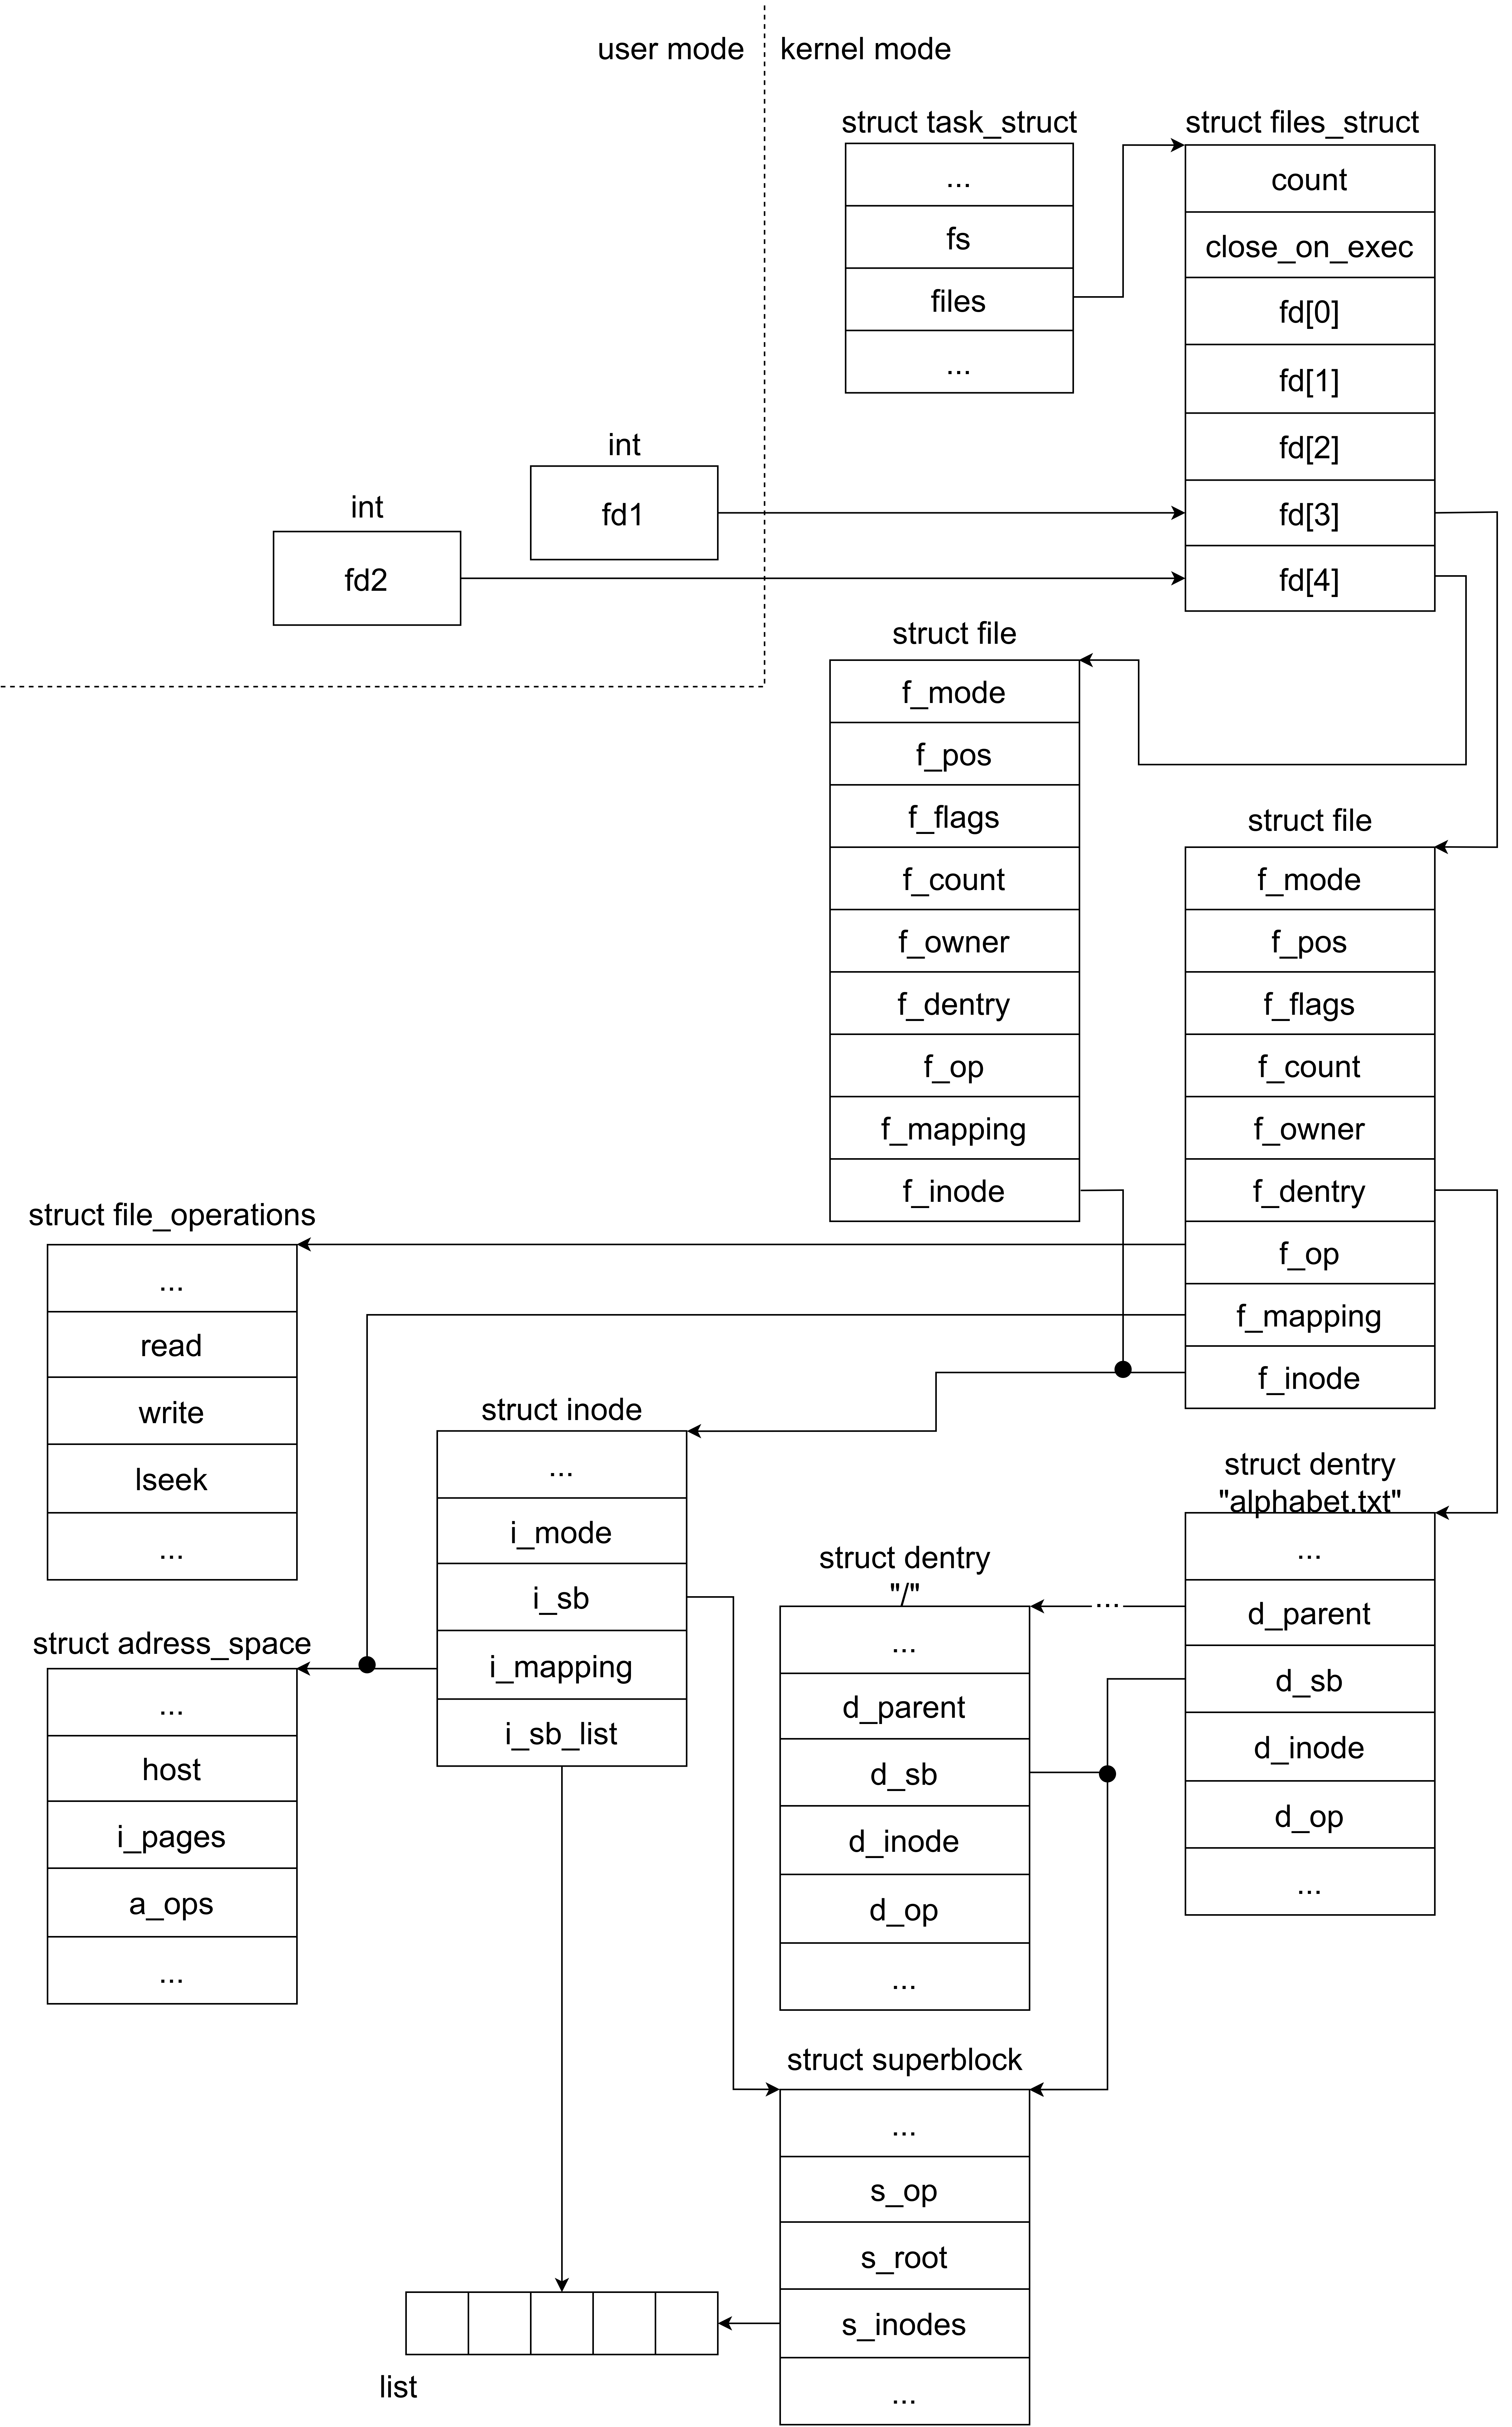
\includegraphics[height=0.91\textheight]{img/structures-2.drawio.png}
	\caption{Связи структур во второй программе}
\end{figure}

\subsection{Многопоточный вариант}

\lstinputlisting[language=C, caption={Вторая программа с созданием одного дополнительного потока}]{../2/1_thread.c}

\begin{lstlisting}[caption={\text{Вывод программы}}]
AbcAdbecfdgehfgihijjkkllmmnnooppqqrrssttuuvvwwxxyyzz
\end{lstlisting}

\lstinputlisting[language=C, caption={Вторая программа с созданием двух дополнительных потоков}]{../2/2_threads.c}

\begin{lstlisting}[caption={\text{Вывод программы}}]
AbcAdbecfdegfhgihjikjkllmmnnooppqqrrstsutvwuxvywzxyz
\end{lstlisting}

В однопоточной программе в цикле каждый символ из файла выводится два раза подряд, а в многопоточной программе порядок вывода символов не определён, так как потоки выполняются параллельно. При этом дополнительный поток начинает вывод позже главного, так как в программе затрачивается время на его создание.

При создании дополнительных потоков связи структур не изменяются, так как ресурсами (в том числе и открытыми файлами) владеет процесс.

\subsection{Многопроцессный вариант}

\lstinputlisting[language=C, caption={Вторая программа с созданием одного дочернего процесса}]{../2/1_subproc.c}

\begin{lstlisting}[caption={\text{Вывод программы}}]
AbcdefAgbhcidejfkglhminjoklpmqnrosptqurvswtxuyvzwxyz
\end{lstlisting}

\lstinputlisting[language=C, caption={Вторая программа с созданием двух дочерних процессов}]{../2/2_subproc.c}

\begin{lstlisting}[caption={\text{Вывод программы}}]
AbcdefghijklAmbncdoepfqgrhsitjukvlwmxnoypzqrstuvwxyz
\end{lstlisting}

В однопроцессной программе в цикле каждый символ из файла выводится два раза подряд, а в многопроцессной программе порядок вывода символов не определён, так как процессы выполняются параллельно. При этом дочерний процесс начинает вывод позже процесса-родителя, так как в программе затрачивается время на его создание.

При создании дочерних процессов связи структур изменяются: у каждого процесса-потомка есть своя структура task\_struct, ссылающаяся на структуру files\_struct, которая содержит одни и те же дескрипторы (наследуются дочерними процессами). Таким образом, процессы работают с одними и теми же структурами struct file.

В результате вывод многопроцессной программы аналогичен выводу многопоточной.



\section{Третья программа}

\subsection{Базовый вариант}

\lstinputlisting[language=C, caption={Третья программа, базовый вариант}]{../3/common_1.c}

\begin{lstlisting}[caption={\text{Вывод программы}}]
$ ./common_1
fopen fs1: inode number = 49463, size = 0 bytes, blksize = 4096
fopen fs2: inode number = 49463, size = 0 bytes, blksize = 4096
fprintf: inode number = 49463, size = 0 bytes, blksize = 4096
fprintf: inode number = 49463, size = 0 bytes, blksize = 4096
fprintf: inode number = 49463, size = 0 bytes, blksize = 4096
fprintf: inode number = 49463, size = 0 bytes, blksize = 4096
fprintf: inode number = 49463, size = 0 bytes, blksize = 4096
fprintf: inode number = 49463, size = 0 bytes, blksize = 4096
fprintf: inode number = 49463, size = 0 bytes, blksize = 4096
fprintf: inode number = 49463, size = 0 bytes, blksize = 4096
fprintf: inode number = 49463, size = 0 bytes, blksize = 4096
fprintf: inode number = 49463, size = 0 bytes, blksize = 4096
fprintf: inode number = 49463, size = 0 bytes, blksize = 4096
fprintf: inode number = 49463, size = 0 bytes, blksize = 4096
fprintf: inode number = 49463, size = 0 bytes, blksize = 4096
fprintf: inode number = 49463, size = 0 bytes, blksize = 4096
fprintf: inode number = 49463, size = 0 bytes, blksize = 4096
fprintf: inode number = 49463, size = 0 bytes, blksize = 4096
fprintf: inode number = 49463, size = 0 bytes, blksize = 4096
fprintf: inode number = 49463, size = 0 bytes, blksize = 4096
fprintf: inode number = 49463, size = 0 bytes, blksize = 4096
fprintf: inode number = 49463, size = 0 bytes, blksize = 4096
fprintf: inode number = 49463, size = 0 bytes, blksize = 4096
fprintf: inode number = 49463, size = 0 bytes, blksize = 4096
fprintf: inode number = 49463, size = 0 bytes, blksize = 4096
fprintf: inode number = 49463, size = 0 bytes, blksize = 4096
fprintf: inode number = 49463, size = 0 bytes, blksize = 4096
fprintf: inode number = 49463, size = 0 bytes, blksize = 4096
fclose fs1: inode number = 49463, size = 13 bytes, blksize = 4096
fclose fs2: inode number = 49463, size = 13 bytes, blksize = 4096
$ cat common_1.txt
bdfhjlnprtvxz
\end{lstlisting}

В программе файл дважды открывается на запись функцией fopen() из библиотеки stdio.h. В системной таблице открытых файлов создаётся два дескриптора struct file, каждый из которых имеет собственный указатель f\_pos, но оба ссылаются на один и тот же inode. С помощью библиотечной функции fprintf() выполняется буферизованный вывод. Буфер создается без явного указания. Существует 3 причины, по которым данные из буфера записываются в файл:

\begin{enumerate}[label*=\arabic*.]
	\item Буфер заполнен.
	\item Вызвана функция fflush() --- принудительная запись.
	\item Вызвана функция close()/fclose().
\end{enumerate}

В данном случае запись в файл происходит в результате вызова функции fclose(). При вызове fclose() для fs1 буфер для fs1 записывается в файл. При вызове fclose() для fs2, все содержимое файла очищается, а в файл записывается содержимое буфера для fs2. В итоге произошла потеря данных, в файле окажется только содержимое буфера для fs2.

\lstinputlisting[language=C, caption={Третья программа, базовый вариант, порядок вызова fclose() изменён}]{../3/common_2.c}

\begin{lstlisting}[caption={\text{Вывод программы}}]
$ ./common_2
fopen fs1: inode number = 49466, size = 0 bytes, blksize = 4096
fopen fs2: inode number = 49466, size = 0 bytes, blksize = 4096
fprintf: inode number = 49466, size = 0 bytes, blksize = 4096
fprintf: inode number = 49466, size = 0 bytes, blksize = 4096
fprintf: inode number = 49466, size = 0 bytes, blksize = 4096
fprintf: inode number = 49466, size = 0 bytes, blksize = 4096
fprintf: inode number = 49466, size = 0 bytes, blksize = 4096
fprintf: inode number = 49466, size = 0 bytes, blksize = 4096
fprintf: inode number = 49466, size = 0 bytes, blksize = 4096
fprintf: inode number = 49466, size = 0 bytes, blksize = 4096
fprintf: inode number = 49466, size = 0 bytes, blksize = 4096
fprintf: inode number = 49466, size = 0 bytes, blksize = 4096
fprintf: inode number = 49466, size = 0 bytes, blksize = 4096
fprintf: inode number = 49466, size = 0 bytes, blksize = 4096
fprintf: inode number = 49466, size = 0 bytes, blksize = 4096
fprintf: inode number = 49466, size = 0 bytes, blksize = 4096
fprintf: inode number = 49466, size = 0 bytes, blksize = 4096
fprintf: inode number = 49466, size = 0 bytes, blksize = 4096
fprintf: inode number = 49466, size = 0 bytes, blksize = 4096
fprintf: inode number = 49466, size = 0 bytes, blksize = 4096
fprintf: inode number = 49466, size = 0 bytes, blksize = 4096
fprintf: inode number = 49466, size = 0 bytes, blksize = 4096
fprintf: inode number = 49466, size = 0 bytes, blksize = 4096
fprintf: inode number = 49466, size = 0 bytes, blksize = 4096
fprintf: inode number = 49466, size = 0 bytes, blksize = 4096
fprintf: inode number = 49466, size = 0 bytes, blksize = 4096
fprintf: inode number = 49466, size = 0 bytes, blksize = 4096
fprintf: inode number = 49466, size = 0 bytes, blksize = 4096
fclose fs2: inode number = 49466, size = 13 bytes, blksize = 4096
fclose fs1: inode number = 49466, size = 13 bytes, blksize = 4096
$ cat common_2.txt
acegikmoqsuwy
\end{lstlisting}

При изменении порядка вызова функций fclose() вывод программы изменился.

\newpage
\subsection{Связи структур}

\begin{figure}[H]
	\centering
	\includegraphics[height=0.91\textheight]{img/structures-3.drawio.png}
	\caption{Связи структур в третьей программе}
\end{figure}

\subsection{Многопоточный вариант}

\lstinputlisting[language=C, caption={Третья программа с созданием одного дополнительного потока}]{../3/1_thread.c}
\lstinputlisting[language=C, caption={Вывод программы}]{../3/1_thread.txt}

\lstinputlisting[language=C, caption={Третья программа с созданием двух дополнительных потоков}]{../3/2_threads.c}
\lstinputlisting[language=C, caption={Вывод программы}]{../3/2_threads.txt}

В многопоточной программе работа с файлом производится аналогично однопоточной программе. Если вызывать fclose() в дополнительном потоке, то порядок вывода символов будет не определён, так как нельзя предсказать заранее, какой поток последним вызовет fclose().

При создании дополнительных потоков связи структур не изменяются, так как ресурсами (в том числе и открытыми файлами) владеет процесс.

\subsection{Многопроцессный вариант}

\lstinputlisting[language=C, caption={Третья программа с созданием одного дочернего процесса}]{../3/1_subproc.c}
\lstinputlisting[language=C, caption={Вывод программы}]{../3/1_subproc.txt}

\lstinputlisting[language=C, caption={Третья программа с созданием двух дочерних процессов}]{../3/2_subproc.c}
\lstinputlisting[language=C, caption={Вывод программы}]{../3/2_subproc.txt}

В многопроцессной программе работа с файлом производится аналогично однопроцессной программе. Если вызывать fclose() в процессах-потомках, то порядок вывода символов будет не определён, так как нельзя предсказать заранее, какой процесс последним вызовет fclose().

В данной программе применение средств взаимоисключения является избыточным, так как каждый процесс записывает данные в собственный буфер, поэтому параллельная запись не приводит к потере данных.

При создании дочерних процессов связи структур изменяются: у каждого процесса-потомка есть своя структура task\_struct, ссылающаяся на структуру files\_struct, которая содержит одни и те же дескрипторы (наследуются дочерними процессами). Таким образом, процессы работают с одними и теми же структурами struct file.



\section{Четвёртая программа}

\subsection{Базовый вариант}

\lstinputlisting[language=C, caption={Четвёртая программа, базовый вариант}]{../4/common_1.c}

\begin{lstlisting}[caption={\text{Вывод программы}}]
$ ./common_1
open fd1: inode number = 49468, size = 0 bytes, blksize = 4096
open fd2: inode number = 49468, size = 0 bytes, blksize = 4096
write: inode number = 49468, size = 1 bytes, blksize = 4096
write: inode number = 49468, size = 1 bytes, blksize = 4096
write: inode number = 49468, size = 2 bytes, blksize = 4096
write: inode number = 49468, size = 2 bytes, blksize = 4096
write: inode number = 49468, size = 3 bytes, blksize = 4096
write: inode number = 49468, size = 3 bytes, blksize = 4096
write: inode number = 49468, size = 4 bytes, blksize = 4096
write: inode number = 49468, size = 4 bytes, blksize = 4096
write: inode number = 49468, size = 5 bytes, blksize = 4096
write: inode number = 49468, size = 5 bytes, blksize = 4096
write: inode number = 49468, size = 6 bytes, blksize = 4096
write: inode number = 49468, size = 6 bytes, blksize = 4096
write: inode number = 49468, size = 7 bytes, blksize = 4096
write: inode number = 49468, size = 7 bytes, blksize = 4096
write: inode number = 49468, size = 8 bytes, blksize = 4096
write: inode number = 49468, size = 8 bytes, blksize = 4096
write: inode number = 49468, size = 9 bytes, blksize = 4096
write: inode number = 49468, size = 9 bytes, blksize = 4096
write: inode number = 49468, size = 10 bytes, blksize = 4096
write: inode number = 49468, size = 10 bytes, blksize = 4096
write: inode number = 49468, size = 11 bytes, blksize = 4096
write: inode number = 49468, size = 11 bytes, blksize = 4096
write: inode number = 49468, size = 12 bytes, blksize = 4096
write: inode number = 49468, size = 12 bytes, blksize = 4096
write: inode number = 49468, size = 13 bytes, blksize = 4096
write: inode number = 49468, size = 13 bytes, blksize = 4096
close fd1: inode number = 49468, size = 13 bytes, blksize = 4096
close fd2: inode number = 49468, size = 13 bytes, blksize = 4096
$ cat common_1.txt
bdfhjlnprtvxz 
\end{lstlisting}

В программе файл дважды открывается на запись функцией open(). В системной таблице открытых файлов создаётся два дескриптора struct file, каждый из которых имеет собственный указатель f\_pos, но оба ссылаются на один и тот же inode. С помощью системного вызова write() выполняется небуферизованный вывод.

При изменении порядка вызова функций close() вывод программы не изменяется, так как вывод не буферизуется.

Чтобы вывести алфавит полностью, можно для второго открытия файла использовать open() с флагом O\_APPEND. В таком случае перед каждым вызовом write() для fd2 указатель f\_pos будет устанавливаться в конце файла, как если бы использовался lseek().

\lstinputlisting[language=C, caption={Четвёртая программа, базовый вариант, использован флаг O\_APPEND}]{../4/common_2.c}

\begin{lstlisting}[caption={\text{Вывод программы}}]
$ ./common_2
open fd1: inode number = 49473, size = 0 bytes, blksize = 4096
open fd2: inode number = 49473, size = 0 bytes, blksize = 4096
write fd1: inode number = 49473, size = 1 bytes, blksize = 4096
write fd1: inode number = 49473, size = 2 bytes, blksize = 4096
write fd1: inode number = 49473, size = 3 bytes, blksize = 4096
write fd1: inode number = 49473, size = 4 bytes, blksize = 4096
write fd1: inode number = 49473, size = 5 bytes, blksize = 4096
write fd1: inode number = 49473, size = 6 bytes, blksize = 4096
write fd1: inode number = 49473, size = 7 bytes, blksize = 4096
write fd1: inode number = 49473, size = 8 bytes, blksize = 4096
write fd1: inode number = 49473, size = 9 bytes, blksize = 4096
write fd1: inode number = 49473, size = 10 bytes, blksize = 4096
write fd1: inode number = 49473, size = 11 bytes, blksize = 4096
write fd1: inode number = 49473, size = 12 bytes, blksize = 4096
write fd1: inode number = 49473, size = 13 bytes, blksize = 4096
write fd2: inode number = 49473, size = 14 bytes, blksize = 4096
write fd2: inode number = 49473, size = 15 bytes, blksize = 4096
write fd2: inode number = 49473, size = 16 bytes, blksize = 4096
write fd2: inode number = 49473, size = 17 bytes, blksize = 4096
write fd2: inode number = 49473, size = 18 bytes, blksize = 4096
write fd2: inode number = 49473, size = 19 bytes, blksize = 4096
write fd2: inode number = 49473, size = 20 bytes, blksize = 4096
write fd2: inode number = 49473, size = 21 bytes, blksize = 4096
write fd2: inode number = 49473, size = 22 bytes, blksize = 4096
write fd2: inode number = 49473, size = 23 bytes, blksize = 4096
write fd2: inode number = 49473, size = 24 bytes, blksize = 4096
write fd2: inode number = 49473, size = 25 bytes, blksize = 4096
write fd2: inode number = 49473, size = 26 bytes, blksize = 4096
close fd1: inode number = 49473, size = 26 bytes, blksize = 4096
close fd2: inode number = 49473, size = 26 bytes, blksize = 4096
$ cat common_2.txt
abcdefghijklmnopqrstuvwxyz
\end{lstlisting}

\newpage
\subsection{Связи структур}

\begin{figure}[H]
	\centering
	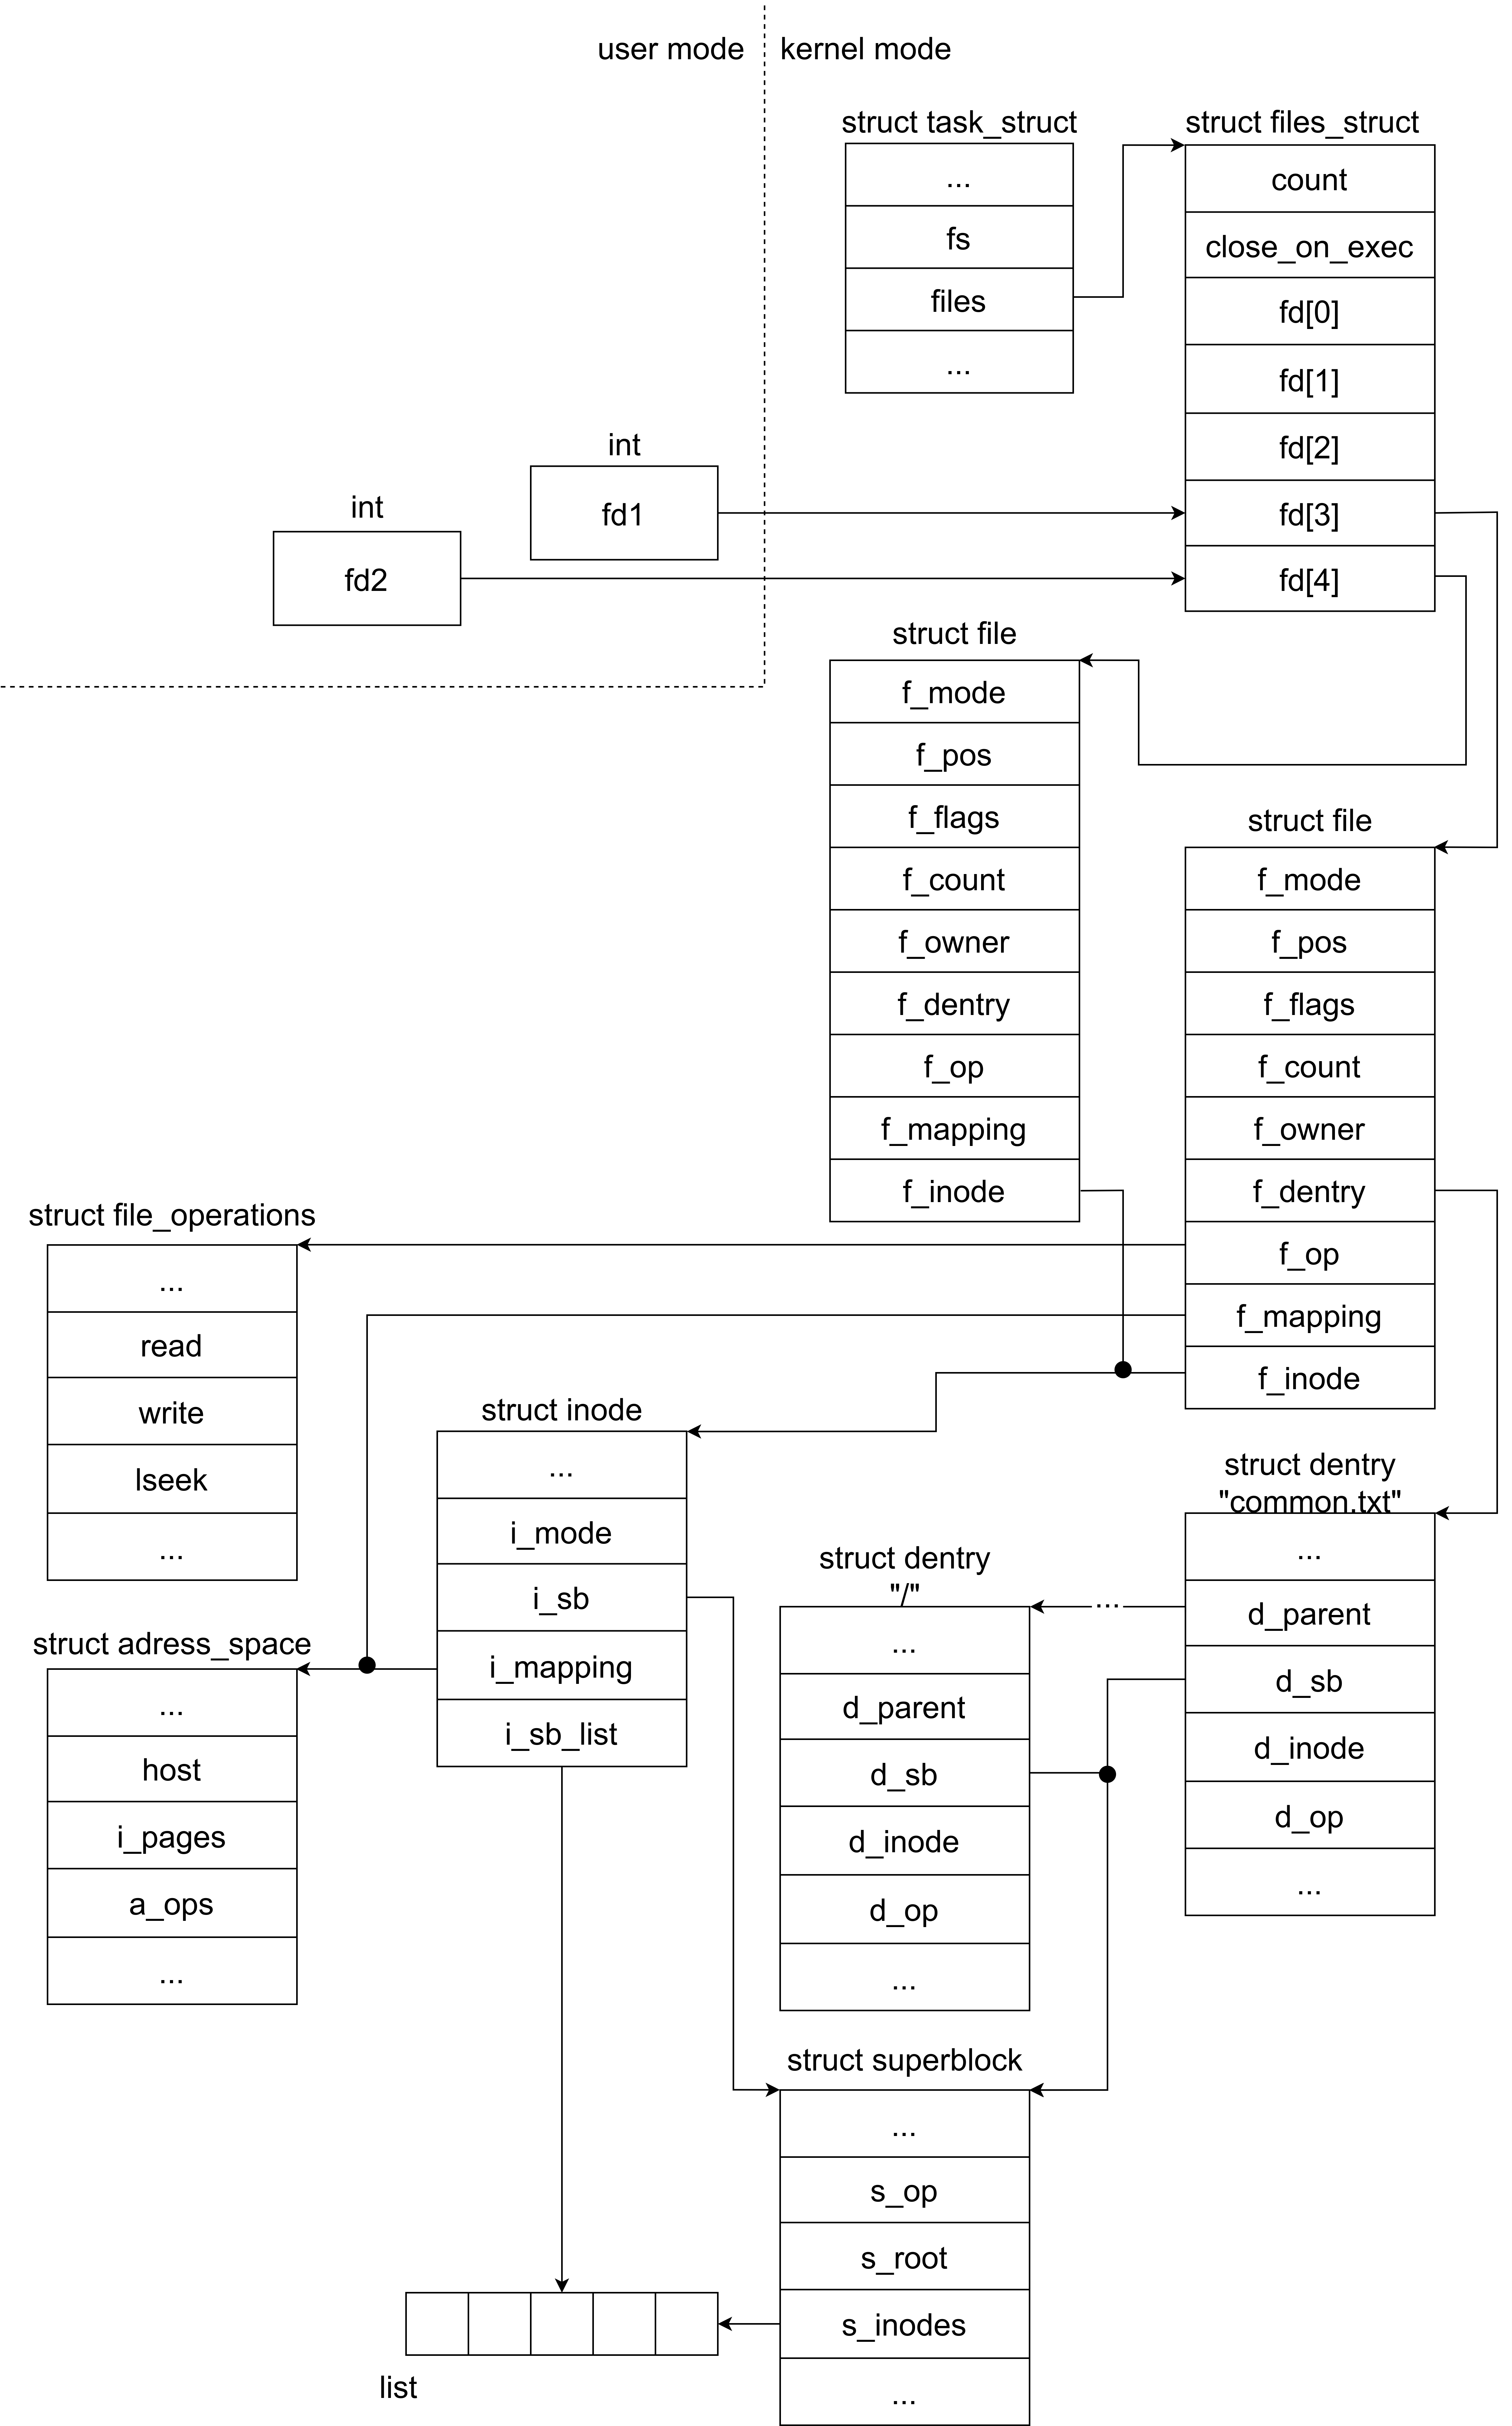
\includegraphics[height=0.91\textheight]{img/structures-4.drawio.png}
	\caption{Связи структур в четвёртой программе}
\end{figure}

\subsection{Многопоточный вариант}

\lstinputlisting[language=C, caption={Четвёртая программа с созданием одного дополнительного потока}]{../4/1_thread.c}
\lstinputlisting[language=C, caption={Вывод программы}]{../4/1_thread.txt}

\lstinputlisting[language=C, caption={Четвёртая программа с созданием двух дополнительных потоков}]{../4/2_threads.c}
\lstinputlisting[language=C, caption={Вывод программы}]{../4/2_threads.txt}

В многопоточной программе работа с файлом производится аналогично однопоточной программе. Если не использовать средства взаимоисключения (например, мьютекс), то вторая половина алфавита будет записываться частично, и поведение программы будет не определено.

При создании дополнительных потоков связи структур не изменяются, так как ресурсами (в том числе и открытыми файлами) владеет процесс.



\end{document}
